% Proposal đồ án, build riêng với báo cáo nhưng dùng chung config/, figures/, references.bib, latexmkrc.
%   cd report && latexmk proposal.tex
% Kết quả: build/proposal.pdf và bản đặt tên theo \TenFilePDFProposal trong config/metadata.tex.
% Nhóm, GVHD, danh sách thành viên: chỉ sửa ở config/metadata.tex.
\documentclass[12pt,a4paper]{report}

% Preamble dùng chung. Biên dịch bằng XeLaTeX (xem latexmkrc).

% --- Ngôn ngữ và phông chữ (Unicode, không cần hack cho tiếng Việt) ---
\usepackage{fontspec}
\usepackage[vietnamese]{babel}
% Chọn font đầu tiên có trên máy: Times New Roman (msttcore-fonts) → Liberation (cùng kích thước,
% có sẵn trên đa số Linux) → TeX Gyre (có trong TeX Live đầy đủ / Overleaf, nạp theo tên file)
% → Latin Modern (mặc định của fontspec, luôn có). Font thực sự được dùng in ra log: tìm "Font chính:".
\newcommand{\chonfont}[4]{% #1 lệnh \set...font, #2 font ưu tiên, #3 font dự phòng, #4 tên file TeX Gyre
  \IfFontExistsTF{#2}{#1{#2}\typeout{Font chính: #2}}{%
    \IfFontExistsTF{#3}{#1{#3}\typeout{Font chính: #3 (thiếu #2)}}{%
      \IfFontExistsTF{#4-regular.otf}{%
        #1{#4}[Extension=.otf, UprightFont=*-regular, BoldFont=*-bold,
               ItalicFont=*-italic, BoldItalicFont=*-bolditalic]%
        \typeout{Font chính: #4 (thiếu #2 và #3)}}{%
        \typeout{Font chính: Latin Modern (thiếu #2, #3, #4)}}}}}
\chonfont{\setmainfont}{Times New Roman}{Liberation Serif}{texgyretermes}
\chonfont{\setsansfont}{Arial}{Liberation Sans}{texgyreheros}
\chonfont{\setmonofont}{Courier New}{Liberation Mono}{texgyrecursor}

% --- Cỡ chữ cố định theo bảng quy ước báo cáo/luận văn ---
% Thân bài 13pt · Mục lớn (section) 14pt · Mục con (subsection) 13pt đậm
% · Chú thích/footnote 10-12pt. Chương và header/listing đặt trực tiếp
% bằng \fontsize tại nơi dùng (xem macros.tex).
\makeatletter
\renewcommand\normalsize{\@setfontsize\normalsize{13}{15.6}} % thân bài: 13pt
\renewcommand\small{\@setfontsize\small{12}{14.4}}           % chú thích bảng/hình: 12pt
\renewcommand\footnotesize{\@setfontsize\footnotesize{10}{12}} % footnote: 10pt
\renewcommand\large{\@setfontsize\large{13}{15.6}}           % tiêu đề mục con (subsection): 13pt
\renewcommand\Large{\@setfontsize\Large{14}{16.8}}           % tiêu đề mục lớn (section): 14pt
\makeatother
\linespread{1.3}  % giãn dòng khoảng 1.5 (chuẩn báo cáo/luận văn)
\setlength{\parindent}{1cm}
\setlength{\parskip}{3pt}

% --- Bố cục: lề trái rộng hơn để đóng gáy ---
\usepackage[a4paper, left=3cm, right=2cm, top=2.5cm, bottom=2.5cm,
            headheight=40pt, headsep=1.0cm]{geometry}
\usepackage{fancyhdr}

% --- Toán, bảng, hình ---
\usepackage{amsmath}
\usepackage{amsthm}     % môi trường định lý / định nghĩa (khai báo ở macros.tex)
\usepackage{unicode-math}
\setmathfont{Latin Modern Math}  % font toán OpenType, chạy mọi cỡ chữ
\usepackage{booktabs, array, tabularx}
\usepackage{graphicx, float, caption}
\usepackage{subcaption}  % nhiều hình con trong một figure
\graphicspath{{figures/}} % \includegraphics tìm ảnh trong figures/
\captionsetup{font=small} % chú thích bảng/hình: 12pt (dùng cỡ \small đã đặt lại ở trên)
\usepackage{xcolor}
\usepackage{colortbl}    % tô màu hàng / ô của bảng
\usepackage{longtable}   % bảng dài tự ngắt trang
\usepackage{siunitx}     % số và đơn vị: \num{}, \SI{}{}, cột S căn theo dấu thập phân
\sisetup{output-decimal-marker={,}, group-separator={.}, group-minimum-digits=4}
\usepackage{algorithm, algorithmic} % khung thuật toán + mã giả
\usepackage{enumerate}
\usepackage[framemethod=tikz]{mdframed}
\usepackage{tikz}
\usetikzlibrary{arrows.meta, positioning}

% --- Mã nguồn ---
\usepackage{listings}

% --- Trích dẫn ---
%% Ghi chú: biblatex khuyến nghị csquotes, nhưng máy chạy lại không cài gói này;
%% thiếu nó chỉ sinh cảnh báo, không ảnh hưởng nội dung.
\usepackage[backend=biber, style=numeric, sorting=none]{biblatex}
\addbibresource{references.bib}
% biblatex không hỗ trợ tiếng Việt: ánh xạ sang tiếng Anh để các chuỗi
% "In:", "et al.", "and" hiện đúng thay vì rơi vào định nghĩa dự phòng hỏng.
\DeclareLanguageMapping{vietnamese}{english}

% --- Siêu liên kết (nạp sau cùng) ---
\usepackage{hyperref}

% Thông tin đề tài: chỉ sửa ở đây, trang bìa và tiêu đề PDF tự cập nhật.
\newcommand{\TenTruong}{Trường Đại học Sài Gòn}
\newcommand{\TenKhoa}{Khoa Công nghệ Thông tin}
\newcommand{\TenMonHoc}{Trí tuệ nhân tạo nâng cao}
\newcommand{\TenDeTai}{Xây dựng và đánh giá Game AI đa cấp độ cho Caro 11×11}
\newcommand{\TenNhom}{Nhóm XX}
\newcommand{\LinkRepo}{https://github.com/SGU-ML25/CaroGame}
\newcommand{\LoaiBaoCao}{Báo cáo đồ án cuối kỳ}
\newcommand{\CommitNop}{chưa chốt}

% Tên file PDF xuất ra cạnh main.tex sau mỗi lần build (không gồm đuôi .pdf; để trống {} thì không xuất).
% Không dùng lệnh LaTeX ở đây, chỉ chữ thường; latexmkrc đọc thẳng dòng này.
\newcommand{\TenFilePDF}{Nhóm XX - Caro 11x11 - TTNTNC}
\newcommand{\TenFilePDFProposal}{Nhóm XX - Caro 11x11 - Proposal}

% Bản nháp / bản nộp. Nháp: dấu mờ "BẢN NHÁP", hiện \goiy và \chualam.
% Nộp (\BanNoptrue): không dấu mờ; còn sót \goiy hoặc \chualam thì build báo lỗi.
\newif\ifBanNop
\BanNopfalse

\newcommand{\GVHD}{(bổ sung)}
\newcommand{\ThoiGian}{TP. Hồ Chí Minh, tháng 12/2026}

% Danh sách sinh viên: mỗi dòng "& Họ tên & MSSV \\" (cột đầu để trống)
\newcommand{\DanhSachSV}{%
  & Huỳnh Thanh Tiến & 3123410374 \\
  & (TV2)            & (MSSV) \\
  & (TV3)            & (MSSV) \\
  & (TV4)            & (MSSV) \\
}

% Macro, màu sắc, thiết lập listings / hyperref / header.

\definecolor{dkgreen}{rgb}{0,0.6,0}
\definecolor{gray}{rgb}{0.5,0.5,0.5}
\definecolor{mauve}{rgb}{0.58,0,0.82}

\hypersetup{
  urlcolor=blue, linkcolor=black, citecolor=black, colorlinks=true,
  pdftitle={\TenDeTai}, pdfauthor={\TenKhoa, \TenTruong},
}

% --- Mã nguồn: listings chỉ dựng bảng ký tự cho mã 0--255. Chữ tiếng Việt có dấu (mã > 255) bị in
% ngay trong khi chữ ASCII còn nằm trong bộ đệm, làm đảo thứ tự ("hoặc" thành "ặhoc"). Hook dưới đây
% đăng ký các chữ đó là chữ cái của listings, giống cách listings tự làm với a--z. ---
\makeatletter
\def\lst@VNletters{258,259,272,273,296,297,360,361,416,417,431,432,7840,7841,7842,7843,7844,7845,7846,7847,7848,7849,7850,7851,7852,7853,7854,7855,7856,7857,7858,7859,7860,7861,7862,7863,7864,7865,7866,7867,7868,7869,7870,7871,7872,7873,7874,7875,7876,7877,7878,7879,7880,7881,7882,7883,7884,7885,7886,7887,7888,7889,7890,7891,7892,7893,7894,7895,7896,7897,7898,7899,7900,7901,7902,7903,7904,7905,7906,7907,7908,7909,7910,7911,7912,7913,7914,7915,7916,7917,7918,7919,7920,7921,7922,7923,7924,7925,7926,7927,7928,7929,9472,9474,9492,9500}
\lst@AddToHook{SelectCharTable}{%
  \@for\lst@vn:=\lst@VNletters\do{%
    \catcode\lst@vn=\active
    \begingroup\lccode`\~=\lst@vn\relax\lccode`\/=\lst@vn\relax
    \lowercase{\endgroup\def~{\lst@ProcessLetter/}}}}
\makeatother

\lstset{
  frame=tb,
  language=Python,
  aboveskip=3mm,
  belowskip=3mm,
  showstringspaces=false,
  columns=flexible,
  basicstyle={\fontsize{10.5}{12.6}\selectfont\ttfamily}, % code/listing: 10.5pt
  numbers=left,
  numberstyle=\tiny\color{gray},
  keywordstyle=\color{blue},
  commentstyle=\color{dkgreen},
  stringstyle=\color{mauve},
  breaklines=true,
  breakatwhitespace=true,
  tabsize=3,
  numbersep=5pt,
  escapeinside={(*@}{@*)},
  captionpos=t
}

% --- Kiểu cho mã LaTeX (dùng trong tài liệu hướng dẫn): \begin{lstlisting}[style=latex] ---
\lstdefinestyle{latex}{language=[LaTeX]TeX, numbers=none, backgroundcolor=\color{gray!8},
  texcsstyle=*\color{blue}, moretexcs={includegraphics,subcaption,caption,label,ref,cite,toprule,midrule,bottomrule,
  multicolumn,rowcolor,cellcolor,num,SI,eqref,goiy,chualam,chuatrienkhai,lstinputlisting,url,href,textcite,
  autoref,cline,addplot,draw,node,STATE,IF,ELSE,ENDIF,FOR,ENDFOR,RETURN,REQUIRE,ENSURE,WHILE,ENDWHILE}}

% --- Định lý / định nghĩa / ví dụ (amsthm), đánh số theo chương ---
\theoremstyle{plain}
\newtheorem{dinhly}{Định lý}[chapter]
\theoremstyle{definition}
\newtheorem{dinhnghia}{Định nghĩa}[chapter]
\newtheorem{vidu}{Ví dụ}[chapter]
\theoremstyle{remark}
\newtheorem*{nhanxet}{Nhận xét}

% --- Tên tiếng Việt cho khung thuật toán ---
\floatname{algorithm}{Thuật toán}
\renewcommand{\algorithmicrequire}{\textbf{Đầu vào:}}
\renewcommand{\algorithmicensure}{\textbf{Đầu ra:}}

% --- Đánh số "Đoạn mã N.M" cho lstlisting, theo chương, giống Bảng/Hình ---
% (listings tự đặt lại số theo chương khi lớp tài liệu có \thechapter)
\renewcommand{\lstlistingname}{Đoạn mã}
\renewcommand{\lstlistlistingname}{Danh sách đoạn mã}

% --- Hộp ghi chú cho phần chưa triển khai ---
\newcommand{\chuatrienkhai}[1]{%
  \begin{mdframed}[backgroundcolor=yellow!15, linecolor=orange, linewidth=1pt]
    \textbf{Chưa triển khai.} #1
  \end{mdframed}}

% --- Ghi chú ngắn cho nội dung sẽ bổ sung ở các tuần sau ---
% --- Gợi ý nội dung cần viết trong sườn bài (xoá khi viết xong mục) ---
% Ở bản nộp (\BanNoptrue trong metadata.tex) cả hai báo lỗi để không nộp sót.
\ifBanNop
  \newcommand{\chualam}[1]{\PackageError{baocao}{Bản nộp còn \string\chualam{#1}}{Viết xong rồi xoá lệnh này.}}
  \newcommand{\goiy}[1]{\PackageError{baocao}{Bản nộp còn \string\goiy{#1}}{Viết xong mục rồi xoá lệnh này.}}
\else
  \newcommand{\chualam}[1]{\textit{(Chưa làm --- #1)}}
  \newcommand{\goiy}[1]{{\color{gray}\itshape [Cần viết: #1]}\par}
\fi

% --- Dấu mờ "BẢN NHÁP" trên mọi trang khi chưa bật \BanNoptrue ---
\ifBanNop\else
  \AddToHook{shipout/background}{%
    \put(0.5\paperwidth,-0.5\paperheight){\makebox(0,0){\rotatebox{45}{%
      \fontsize{90}{90}\selectfont\bfseries\color{gray!12}BẢN NHÁP}}}}
\fi

% --- Logo: bỏ qua êm nếu chưa có file figures/logoITSGU.png ---
\newcommand{\logo}[1]{\IfFileExists{figures/logoITSGU.png}%
  {
\includegraphics[#1]{figures/logoITSGU.png}}{}}

% --- Header / footer ---
\setlength{\headheight}{40pt}
\renewcommand{\headrule}{\vskip 2pt\hrule height 0.4pt\vskip 0pt}
\pagestyle{fancy}
\fancyhf{}
\fancyhead[L]{%
  \begin{tabular}{rl}
    \begin{picture}(25,15)(0,0)
      \put(0,-8){\logo{width=8mm,height=8mm}}
    \end{picture} &
    \begin{tabular}[c]{l}
      \normalfont\fontsize{11}{13}\selectfont \TenTruong \\ \TenKhoa % header: 11pt
    \end{tabular}
  \end{tabular}}
\fancyfoot[C]{\thepage}
\renewcommand{\headrulewidth}{0.4pt}
% Trang mở đầu chương dùng cùng kiểu header
\fancypagestyle{plain}{\pagestyle{fancy}}

\setcounter{secnumdepth}{3}
\setcounter{tocdepth}{2}

% --- Tiêu đề chương: căn giữa, in hoa, đậm, một dòng "CHƯƠNG N. TÊN" ---
\makeatletter
\def\@makechapterhead#1{%
  {\parindent\z@ \centering \normalfont\fontsize{17}{20}\selectfont\bfseries % tiêu đề chương: 17pt
   \MakeUppercase{\@chapapp\ \thechapter.\ #1}\par\nobreak
   \vskip 18\p@}}
\def\@makeschapterhead#1{%
  {\parindent\z@ \centering \normalfont\fontsize{17}{20}\selectfont\bfseries % tiêu đề chương: 17pt
   \MakeUppercase{#1}\par\nobreak
   \vskip 18\p@}}
\makeatother

% --- \texttt cho phép xuống dòng sau / _ . để tên file không tràn lề ---
\let\oldtexttt\texttt
\ExplSyntaxOn
\tl_new:N \l__tt_break_tl
\RenewDocumentCommand{\texttt}{m}
  {
    \tl_set:Nn \l__tt_break_tl {#1}
    \tl_replace_all:Nnn \l__tt_break_tl { \_ } { \_ \allowbreak }
    \tl_replace_all:Nnn \l__tt_break_tl { / } { / \allowbreak }
    \tl_replace_all:Nnn \l__tt_break_tl { . } { . \allowbreak }
    \tl_replace_all:Nnn \l__tt_break_tl { - } { - \allowbreak }
    \exp_args:NV \oldtexttt \l__tt_break_tl
  }
\ExplSyntaxOff
\emergencystretch=2em

% --- Từ khoá tiếng Việt cho mã giả (algorithmic) ---
\renewcommand{\algorithmicif}{\textbf{nếu}}
\renewcommand{\algorithmicthen}{\textbf{thì}}
\renewcommand{\algorithmicelse}{\textbf{ngược lại}}
\renewcommand{\algorithmicend}{\textbf{hết}}
\renewcommand{\algorithmicfor}{\textbf{với}}
\renewcommand{\algorithmicdo}{\textbf{làm}}
\renewcommand{\algorithmicwhile}{\textbf{trong khi}}
\renewcommand{\algorithmicreturn}{\textbf{trả về}}

% --- Tên lệnh LaTeX trong bảng / chú thích: \cmd{goiy\{...\}} → \goiy{...} ---
\newcommand{\cmd}[1]{\texttt{\textbackslash #1}}



% --- Điều chỉnh riêng cho proposal: chữ nhỏ và lề hẹp hơn báo cáo, không có chương, không dấu "BẢN NHÁP" ---
\RemoveFromHook{shipout/background}[top-level]
\geometry{left=2.2cm, right=2cm, top=2.4cm, bottom=2cm, headheight=40pt, headsep=0.5cm}
\setlength{\headwidth}{\textwidth}
\makeatletter
\renewcommand\normalsize{\@setfontsize\normalsize{12}{14.4}}
\renewcommand\small{\@setfontsize\small{10.5}{12.6}}
\def\@seccntformat#1{\csname the#1\endcsname.\quad}
\makeatother
\normalsize
\linespread{1.12}
\setlength{\parindent}{0pt}
\setlength{\parskip}{4pt}

\renewcommand{\thesection}{\arabic{section}}
\renewcommand{\thefigure}{\arabic{figure}}
\renewcommand{\thetable}{\arabic{table}}
\AtBeginDocument{\renewcommand{\thelstlisting}{\arabic{lstlisting}}}
\captionsetup{font={small,it}, labelfont={bf,up}}
\hypersetup{pdftitle={Proposal đồ án cuối kỳ: Game AI đa cấp độ, Caro 11×11 (\TenNhom)}}

\fancyfoot[C]{\small Proposal -- Game AI Caro 11×11 -- Trang \thepage}

\usetikzlibrary{calc, fit, shapes.misc}
\definecolor{xanhdam}{HTML}{0B4A7C}
\definecolor{xanhnhat}{HTML}{E4EEF6}
\definecolor{quanx}{HTML}{1E293B}
\definecolor{quano}{HTML}{C81E1E}
\definecolor{ovang}{HTML}{FDE68A}
\definecolor{luc}{HTML}{1B7F4B}
\definecolor{cam}{HTML}{B65C00}

\newenvironment{gon}{\begin{itemize}\setlength{\itemsep}{2pt}\setlength{\parskip}{0pt}}{\end{itemize}}

% Bàn cờ TikZ: ô (r, c) có tâm tại (c+.5, -(r+.5))
\newcommand{\luoi}[1]{\draw[gray!55, line width=.3pt] (0,0) grid (#1,-#1); \draw[gray!90] (0,0) rectangle (#1,-#1);}
\newcommand{\chuX}[2]{\node[text=quanx, font=\bfseries] at (#2+.5,-#1-.5) {X};}
\newcommand{\chuO}[2]{\node[text=quano, font=\bfseries] at (#2+.5,-#1-.5) {O};}
\newcommand{\toO}[2]{\fill[ovang] (#2,-#1) rectangle ++(1,-1);}
\newcommand{\dX}[2]{\fill[quanx] (#2+.5,-#1-.5) circle (.36);}
\newcommand{\dO}[2]{\fill[quano] (#2+.5,-#1-.5) circle (.36);}
\newcommand{\oThang}[2]{\draw[luc, line width=1pt] (#2+.5,-#1-.5) circle (.34); \fill[luc] (#2+.5,-#1-.5) circle (.1);}
\newcommand{\tenhinh}[2]{\node[anchor=south, font=\footnotesize\bfseries, align=center] at (3.5,0.1) {#1}; \node[anchor=north, font=\footnotesize, align=center] at (3.5,-7.1) {#2};}

\begin{document}

% ============================== TRANG BÌA ==============================
\begin{titlepage}
  \thispagestyle{empty}
  \begin{tikzpicture}[remember picture, overlay]
    \draw[xanhdam, line width=1pt]
      ($(current page.north west)+(1.3cm,-1.3cm)$) rectangle ($(current page.south east)+(-1.3cm,1.3cm)$);
  \end{tikzpicture}\par
  \centering
  \vspace*{1cm}
  {\fontsize{18}{22}\selectfont\bfseries\color{xanhdam} PROPOSAL ĐỒ ÁN CUỐI KỲ\par}
  \vspace{4pt}
  {\fontsize{14}{17}\selectfont\itshape\color{xanhdam} \TenMonHoc\par}
  \vspace{1.4cm}
  \logo{width=4.2cm}\par
  \vspace{1.6cm}
  {\fontsize{14}{17}\selectfont\bfseries ĐỀ TÀI\par}
  \vspace{6pt}
  {\fontsize{19}{24}\selectfont\bfseries\color{xanhdam} XÂY DỰNG VÀ ĐÁNH GIÁ GAME AI ĐA CẤP ĐỘ\par}
  \vspace{6pt}
  {\fontsize{14}{17}\selectfont\itshape Trường hợp nghiên cứu: Caro 11×11 (luật tự do, 5 quân liên tiếp là thắng)\par}
  \vspace{1.6cm}
  {\bfseries GV HƯỚNG DẪN: \GVHD\par}
  \vspace{4pt}
  {\bfseries \MakeUppercase{\TenNhom}: CARO 11×11\par}
  \vspace{4pt}
  {\bfseries THÀNH VIÊN THAM GIA:\par}
  \vspace{2pt}
  \begin{tabular}{@{}l l l@{}}
    \DanhSachSV
  \end{tabular}\par
  \vspace{10pt}
  {\small \TenKhoa, \TenTruong\\ Mã nguồn: \url{\LinkRepo}\par}
  \vfill
  {\small\itshape Proposal -- Game AI Caro 11×11 -- Trang 1\par}
\end{titlepage}
\setcounter{page}{2}

% ============================== TÓM TẮT ==============================
\section*{TÓM TẮT ĐỀ TÀI}
\hrule\vspace{4pt}

Đề tài chọn trò chơi Caro (Gomoku) trên bàn 11×11, luật tự do, làm môi trường thực nghiệm để cài đặt và đánh giá một chuỗi tác tử trí tuệ nhân tạo tăng dần về độ phức tạp phương pháp:
\textbf{Random (Cấp 1) $\rightarrow$ Rule-based P1--P7 (Cấp 2) $\rightarrow$ Negamax Alpha-Beta (Cấp 3) $\rightarrow$ MCTS-UCT (Cấp 4) $\rightarrow$ Policy học có giám sát (Cấp 5) $\rightarrow$ REINFORCE có baseline (Cấp 6) $\rightarrow$ PUCT với mạng cấp 5, AlphaGo-inspired (Cấp 7) $\rightarrow$ vòng lặp self-play, AlphaZero-inspired (Cấp 8)}.

Hệ thống gồm: (1) Game Engine tự cài đặt bằng bitboard, mỗi bên là một số nguyên 121 bit, kiểm tra thắng chỉ tốn 3 phép dịch bit cho mỗi hướng; (2) giao diện web FastAPI phục vụ thi đấu người--máy, máy--máy, xem lại ván từ log và hiển thị ``AI đang nghĩ gì''; (3) khung giải đấu vòng tròn 200 ván/cặp từ 100 khai cuộc có đổi màu, hai chế độ ngân sách tính toán, khoảng tin cậy Wilson 95\%, cùng config, seed và log đủ để chạy lại mọi kết quả.

Nghiên cứu trả lời định lượng 4 câu hỏi: \textit{(1) cùng thời gian mỗi nước, MCTS có thắng nhiều hơn Alpha-Beta không; (2) self-play có cải thiện tác tử học được so với mô hình bắt chước chuyên gia không; (3) cắt tỉa và sắp xếp nước giảm chi phí bao nhiêu mà vẫn giữ nguyên giá trị tìm kiếm; (4) lợi thế đi trước trên bàn 11×11 lớn đến mức nào.}

% ============================== 1 ==============================
\section{GIỚI THIỆU VÀ LÀM RÕ ĐỀ TÀI}

\subsection{Bối cảnh nghiên cứu}
Trò chơi hai người có thông tin đầy đủ là môi trường thử nghiệm kinh điển của trí tuệ nhân tạo, từ tìm kiếm đối kháng có cắt tỉa \cite{russell2021aima,knuth1975alphabeta} đến AlphaGo \cite{silver2016alphago} và AlphaZero \cite{silver2018alphazero} kết hợp mạng nơ-ron với tìm kiếm cây Monte Carlo. Xây dựng nhiều tác tử trên cùng một trò chơi cho phép so sánh công bằng giữa tri thức do con người lập trình (luật, hàm lượng giá, tìm kiếm) và tri thức do mô hình tự học.

Caro 11×11 có cận trên không gian trạng thái $3^{121} \approx 5{,}4 \cdot 10^{57}$; chỉ tính các thế có số quân hợp lệ thì còn khoảng $4{,}8 \cdot 10^{56}$, và số chuỗi nước đi không vượt quá $121! \approx 8{,}1 \cdot 10^{200}$. Không gian này đủ lớn để loại bỏ cách làm bảng (Q-learning dạng bảng) và để các thuật toán phân hoá rõ, trong khi toàn bộ bàn cờ vẫn vừa một thanh ghi 128 bit nên có thể chạy hàng nghìn ván trên máy cá nhân. Allis đã chứng minh Gomoku luật tự do trên bàn 15×15 là thắng cho người đi trước \cite{allis1994}; đề tài không giả định kết quả lý thuyết nào cho bàn 11×11 mà đo lợi thế này bằng thực nghiệm. Mọi kết luận chỉ là sức mạnh thực nghiệm trong bộ khai cuộc và ngân sách đã chọn, không phải chơi tối ưu.

\subsection{Luật chơi và cơ chế trò chơi (giải thích trực quan)}
Để người chưa từng chơi Caro cũng nắm được bài toán, luật áp dụng trong đề tài được tóm tắt ở Hình~\ref{fig:luat}.

\begin{figure}[t]
  \centering
  \begin{minipage}[c]{.47\textwidth}
    \centering
    \begin{tikzpicture}[x=.56cm, y=.56cm]
      \foreach \i in {3,...,7} {\toO{\i}{\i}}
      \luoi{11}
      \foreach \c [count=\n from 0] in {A,...,K} {\node[font=\footnotesize, text=gray] at (\n+.5,.4) {\c};}
      \foreach \r in {1,...,11} {\node[font=\footnotesize, text=gray] at (-.5,-\r+.5) {\r};}
      \chuX{5}{5}\chuO{2}{2}\chuX{4}{4}\chuO{8}{8}\chuX{6}{6}\chuO{3}{7}\chuX{3}{3}\chuO{7}{3}\chuX{7}{7}
    \end{tikzpicture}
  \end{minipage}\hfill
  \begin{minipage}[c]{.5\textwidth}
    \small
    \textbf{\color{xanhdam} CƠ CHẾ CARO 11×11 LUẬT TỰ DO}\par\medskip
    \textbf{Đi tự do:} chọn bất kỳ ô trống nào trong 121 ô; không có trọng lực như Connect Four.\par\smallskip
    \textbf{Luân phiên:} X đi trước, O đi sau, mỗi lượt một quân.\par\smallskip
    \textbf{Thắng:} bên đầu tiên có từ 5 quân liên tiếp trở lên theo hàng ngang, cột dọc hoặc đường chéo. Dãy bị chặn hai đầu và dãy dài hơn 5 quân vẫn thắng.\par\smallskip
    \textbf{Hoà:} bàn đầy sau 121 nước (X 61, O 60) mà không bên nào có 5 quân liên tiếp.
  \end{minipage}
  \caption{Một ván kết thúc trên bàn 11×11: X thắng bằng dãy chéo D4--H8 dù O đã chặn cả hai đầu (C3 và I9), điều mà luật ``chặn 2 đầu'' sẽ không công nhận.}
  \label{fig:luat}
\end{figure}

\textbf{1. Không gian nước đi:} Khác với Connect Four chỉ có 7 cột để chọn, ván Caro bắt đầu với 121 nước hợp lệ và giảm dần. Vì đi xa mọi quân hầu như không bao giờ tốt, các tác tử cấp 2--4 chỉ xét ô trống trong bán kính 2 quanh quân đã có, còn khoảng vài chục ứng viên.

\textbf{2. Cửa sổ thắng:} Toàn bàn có đúng 252 cửa sổ 5 ô thẳng hàng: 77 ngang, 77 dọc và 49 cho mỗi đường chéo (Hình~\ref{fig:mau}, hàng trên). Không có luật chặn hai đầu nên chỉ cần xét bên trong cửa sổ: cửa sổ có 4 quân mình và 1 ô trống luôn là một ô thắng ngay.

\begin{figure}[H]
  \centering
  \begin{tikzpicture}[x=.29cm, y=.29cm]
    \begin{scope}[shift={(0,0)}]    \tenhinh{Ngang}{77 cửa sổ}  \luoi{7} \foreach \c in {1,...,5} {\dX{3}{\c}} \end{scope}
    \begin{scope}[shift={(10,0)}]   \tenhinh{Dọc}{77 cửa sổ}    \luoi{7} \foreach \r in {1,...,5} {\dX{\r}{3}} \end{scope}
    \begin{scope}[shift={(20,0)}]   \tenhinh{Chéo xuống phải}{49 cửa sổ} \luoi{7} \foreach \i in {1,...,5} {\dX{\i}{\i}} \end{scope}
    \begin{scope}[shift={(30,0)}]   \tenhinh{Chéo xuống trái}{49 cửa sổ} \luoi{7} \foreach \i in {1,...,5} {\dX{\i}{6-\i}} \end{scope}
    \begin{scope}[shift={(4,-13)}]  \tenhinh{Tứ bị chặn}{1 ô thắng:\\đối thủ phải chặn} \luoi{7} \foreach \c in {1,...,4} {\dX{3}{\c}} \dO{3}{0} \oThang{3}{5} \end{scope}
    \begin{scope}[shift={(15,-13)}] \tenhinh{Tứ mở}{2 ô thắng:\\không chặn nổi} \luoi{7} \foreach \c in {1,...,4} {\dX{3}{\c}} \oThang{3}{0} \oThang{3}{5} \end{scope}
    \begin{scope}[shift={(26,-13)}] \tenhinh{Tứ kép}{2 ô thắng:\\không chặn nổi} \luoi{7} \foreach \c in {1,...,4} {\dX{3}{\c}} \dX{1}{4}\dX{2}{4}\dX{4}{4}\dO{3}{0}\dO{0}{4} \oThang{3}{5}\oThang{5}{4} \end{scope}
  \end{tikzpicture}
  \caption{Hàng trên: bốn hướng tạo dãy thắng và số cửa sổ 5 ô trên bàn 11×11. Hàng dưới: các thế đe doạ (chấm đen X, chấm đỏ O, vòng xanh là ô thắng ngay của X); số ô thắng đã được đối chiếu bằng hàm \texttt{winning\_squares} của engine.}
  \label{fig:mau}
\end{figure}

\textbf{3. Các tình huống chiến thuật tiêu biểu:}
\begin{gon}
  \item \textbf{Kiểm soát trung tâm:} ô tâm F6 thuộc 20 trong 252 cửa sổ, trong khi ô giữa cạnh chỉ thuộc 8 và ô góc chỉ thuộc 3. Vì vậy bàn trống thì tác tử đi vào tâm.
  \item \textbf{Nước ép (tứ):} tạo 4 quân trong một cửa sổ còn sống buộc đối thủ phải chặn ngay. Chuỗi tứ liên tiếp dẫn tới thắng (VCF) là chỗ tác tử chỉ nhìn 1 nước không nhận ra được.
  \item \textbf{Đòn kép:} sau nước đi của mình, nếu có từ 2 ô thắng ngay và đối thủ không có ô thắng nào thì mình chắc thắng, vì mỗi lượt đối thủ chỉ chặn được một ô (Hình~\ref{fig:mau}). Nhận diện và tạo đòn kép là thước đo rõ nhất của độ sâu chiến thuật.
\end{gon}

\begin{figure}[H]
  \centering
  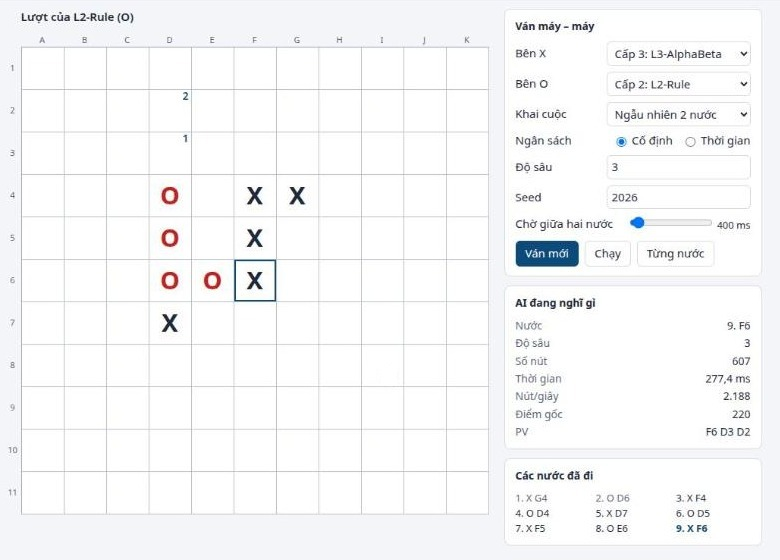
\includegraphics[width=.8\textwidth]{ui-may-may.jpg}
  \caption{Giao diện web của nhóm (\texttt{caro/ui/}) ở chế độ máy--máy: Cấp 3 độ sâu 3 đấu Cấp 2, kèm khung ``AI đang nghĩ gì'' (độ sâu, số nút, thời gian, PV; số 1, 2 trên bàn là các nước kế tiếp trong PV). Đây là ảnh một ván chạy thử, không phải số liệu thực nghiệm.}
  \label{fig:ui}
\end{figure}

\subsection{Mô hình hoá toán học trò chơi}
Caro là trò chơi hai người, quan sát đầy đủ, tất định, tổng bằng không, được hình thức hoá như sau:
\begin{gon}
  \item \textbf{Trạng thái ($S$):} $s = (X, O, \textit{side}, \textit{history})$, gồm hai bitboard 121 bit, bên đến lượt và danh sách nước đã đi. Mạng nơ-ron nhận tensor $\mathbf{x} \in \{0,1\}^{4 \times 11 \times 11}$ nhìn từ góc bên đang đi: quân mình, quân đối thủ, nước vừa đi và một lớp toàn 1.
  \item \textbf{Hành động ($A$):} $A = \{0, \dots, 120\}$ với ô $(r, c)$ ứng với $i = 11r + c$. $\text{Legal}(s)$ là tập ô trống, và rỗng khi ván đã kết thúc; nước bất hợp lệ bị engine từ chối (\texttt{IllegalMoveError}).
  \item \textbf{Hàm chuyển ($T$):} $T(s, a) \rightarrow s'$ tất định: đặt quân vào ô $a$, đổi lượt, rồi kiểm tra kết thúc trên bitboard của người vừa đi.
  \item \textbf{Phần thưởng ($R$):} thưa, chỉ có ở cuối ván, theo góc nhìn từng người chơi: $+1$ thắng, $-1$ thua, $0$ hoà và $0$ ở mọi bước giữa ván; học tăng cường dùng $\gamma = 1$ vì ván có độ dài hữu hạn.
\end{gon}
{\sloppy API thống nhất cho mọi tác tử, arena và giao diện: \texttt{reset()}, \texttt{legal\_actions()}, \texttt{step(action)}, \texttt{is\_terminal()}, \texttt{result()}, \texttt{render()}, \texttt{clone()}/\texttt{undo()}.\par}

\subsection{Phạm vi và phần kế thừa}
Bắt buộc: engine, giao diện, tác tử cấp 1--4, tối thiểu một tác tử học được; nhóm đặt mục tiêu làm cả cấp 5 và 6, còn cấp 7--8 là phần khuyến khích và là bản mô phỏng cảm hứng ở quy mô nhỏ, không khẳng định tái hiện AlphaGo/AlphaZero. Nhóm tự cài đặt engine, tác tử, arena và giao diện; phần kế thừa gồm thư viện (NumPy, PyTorch, FastAPI, \texttt{huggingface\_hub}) và các nguồn ở mục~\ref{sec:tltk}. Công cụ AI đã dùng sẽ được khai báo trong báo cáo cuối kỳ theo quy định của đề.

% ============================== 2 ==============================
\section{MỤC TIÊU VÀ CÂU HỎI NGHIÊN CỨU}

\subsection{Phân cấp mục tiêu nghiên cứu}
Nhóm cấu trúc thành 3 \textbf{mục tiêu chiến lược}, liên kết kỹ thuật nền tảng, thuật toán và phương pháp đánh giá. Các ngưỡng ở cột cuối là chỉ tiêu đặt ra trước khi chạy, chưa phải kết quả.

{\small\setlength{\LTpre}{4pt}\setlength{\LTpost}{4pt}
\begin{longtable}{@{}p{.2\textwidth} p{.39\textwidth} p{.36\textwidth}@{}}
  \toprule
  \textbf{Mục tiêu cấp 1} & \textbf{Mục tiêu cấp 2 (nhiệm vụ)} & \textbf{Tiêu chí hoàn thành} \\
  \midrule\endhead
  \textbf{MỤC TIÊU 1} Hạ tầng engine và môi trường mô phỏng trực quan
  & \textbf{1.1. Engine bitboard:} hai số 121 bit, kiểm tra thắng và tìm ô thắng ngay bằng phép bit.
  & \texttt{has\_five}, \texttt{winning\_squares}, \texttt{candidates} khớp bản duyệt mảng trên bàn ngẫu nhiên; ruff và pytest xanh trên CI. \\
  \cmidrule{2-3}
  & \textbf{1.2. Kiểm chuẩn cây trò chơi (perft):} đếm chuỗi nước từ bàn trống.
  & Trước nước thứ 9 chưa ai có thể có 5 quân, nên độ sâu $d \le 8$ phải đúng $121!/(121-d)!$; ví dụ $d = 3$: \num{1727880}. \\
  \cmidrule{2-3}
  & \textbf{1.3. Giao diện:} FastAPI + trang web cho người--máy, máy--máy, xem lại.
  & Chọn được mọi cấp đã cài; lùi nước; từ chối nước sai (HTTP 400); mở lại ván bất kỳ từ log; hiện độ sâu, số nút, PV, bản đồ nhiệt. \\
  \midrule
  \textbf{MỤC TIÊU 2} Hiện thực hệ tác tử đa cấp độ
  & \textbf{2.1. Cấp 1--3:} Random, luật P1--P7, Negamax Alpha-Beta có iterative deepening, bảng chuyển vị, sắp xếp nước.
  & Cấp 2--3 luôn đi nước thắng ngay và chặn ô thắng duy nhất của đối thủ; Alpha-Beta cho cùng giá trị gốc với bản tắt cắt tỉa và giảm $\ge 70\%$ số nút ở độ sâu 3. \\
  \cmidrule{2-3}
  & \textbf{2.2. Cấp 4:} MCTS-UCT đủ 4 bước, rollout ngẫu nhiên và rollout nhẹ có luật.
  & Score trước Cấp 1 $\ge 0{,}95$ ở \num{1600} mô phỏng; có đường score theo số mô phỏng (100 đến \num{6400}). \\
  \cmidrule{2-3}
  & \textbf{2.3. Cấp 5--6:} ResNet policy-value học từ dữ liệu chuyên gia; REINFORCE có baseline.
  & Thực sự huấn luyện, có checkpoint và seed; báo cáo top-1/top-3 trên tập test tách theo ván; learning curve theo episode so với đối thủ cố định. \\
  \cmidrule{2-3}
  & \textbf{2.4. Cấp 7--8 (khuyến khích):} PUCT với mạng cấp 5; vòng lặp self-play có gating.
  & Bảng thành phần đã/chưa cài; checkpoint mới chỉ thay bản tốt nhất khi score $\ge 55\%$ qua 100 ván đổi màu. \\
  \midrule
  \textbf{MỤC TIÊU 3} Chuẩn mực thực nghiệm đối kháng và khả năng tái lập
  & \textbf{3.1. Giải round-robin:} 8 tác tử, 28 cặp, 200 ván/cặp, 100 khai cuộc đổi màu, 2 chế độ ngân sách.
  & Ma trận score kèm khoảng tin cậy Wilson 95\% cho mỗi chế độ; khác biệt nằm trong khoảng tin cậy được báo cáo là chưa phân biệt được. \\
  \cmidrule{2-3}
  & \textbf{3.2. Ablation:} A1--A7, A5b và E3 (Bảng~\ref{tab:ablation}); đề yêu cầu tối thiểu 2.
  & Bắt buộc A1, A3; trả lời đủ RQ1--RQ4 bằng số liệu, thiếu dữ liệu thì ghi rõ chưa kết luận được. \\
  \cmidrule{2-3}
  & \textbf{3.3. Tái lập:} config, seed, commit và log thô cho mọi lần chạy.
  & Mọi bảng và hình trong báo cáo sinh lại được bằng notebook từ log đã commit; không chép số tay. \\
  \bottomrule
\end{longtable}}

\subsection{Các câu hỏi nghiên cứu (Research Questions)}
Giả thuyết dưới đây là dự đoán cần kiểm chứng, không phải kết luận.
\begin{gon}
  \item \textbf{RQ1 (Alpha-Beta và MCTS):} Trong cùng thời gian mỗi nước, MCTS (UCT) có thắng nhiều hơn Alpha-Beta không? \textit{Giả thuyết:} Alpha-Beta có hàm lượng giá theo cửa sổ và nước bắt buộc sẽ mạnh hơn MCTS rollout ngẫu nhiên, vì Caro có nhiều đòn ngắn mà rollout ngẫu nhiên khó thấy. \textit{Đo:} score và khoảng Wilson 95\% ở 3 mức thời gian (đề xuất 200, 500 và \num{1000} ms); A3, A4.
  \item \textbf{RQ2 (Self-play và bắt chước):} Self-play (cấp 6, 8) có cải thiện so với mô hình bắt chước chuyên gia (cấp 5) không? \textit{Giả thuyết:} có, nhưng chỉ khi đủ số ván; với ngân sách nhỏ có thể chưa vượt cấp 5. \textit{Đo:} learning curve so với đối thủ cố định, score cấp 6/8 trước cấp 5; A5, A5b.
  \item \textbf{RQ3 (Cắt tỉa và sắp xếp nước):} Cắt tỉa alpha-beta và sắp xếp nước giảm chi phí bao nhiêu mà vẫn giữ nguyên nước chọn? \textit{Giả thuyết:} số nút giảm mạnh dần khi độ sâu tăng, giá trị gốc không đổi. \textit{Đo:} số nút, thời gian, tỷ lệ chọn cùng nước; A1, A2.
  \item \textbf{RQ4 (Lợi thế đi trước):} Lợi thế đi trước trên 11×11 lớn đến mức nào giữa các tác tử cùng cấp? \textit{Giả thuyết:} bên đi trước có score $> 0{,}5$ và lợi thế tăng theo sức mạnh tác tử. \textit{Đo:} score bên đi trước khi từng cấp tự đấu; E3.
\end{gon}

% ============================== 3 ==============================
\section{CƠ SỞ LÝ THUYẾT VÀ PHƯƠNG PHÁP TRIỂN KHAI TÁC TỬ}

\subsection{Nhóm tác tử quy ước và tìm kiếm cổ điển (Cấp 1--4)}
\begin{gon}
  \item \textbf{Cấp 1 -- Random:} chọn đều trên $\text{Legal}(s)$ bằng RNG có seed, làm mốc so sánh tối thiểu.
  \item \textbf{Cấp 2 -- Rule-based:} nhìn trước đúng 1 nước, theo thứ tự ưu tiên: (P1) thắng ngay; (P2) chặn thua ngay; (P3) tạo đòn kép; (P4) phá đòn kép của đối thủ; (P5) tạo tứ; (P6) điểm vị trí; (P7) hoà điểm thì chọn gần tâm, rồi ngẫu nhiên theo seed. \textit{Xung đột luật:} P3 đứng trước P4 vì khi tới P3 đối thủ chắc chắn chưa có ô thắng ngay, nên đòn kép của mình thắng trước; P4 đứng trước P5 vì tạo tứ chỉ ép được một nước, sau đó đối thủ vẫn tạo được đòn kép.
  \item \textbf{Cấp 3 -- Negamax Alpha-Beta \cite{knuth1975alphabeta}:} tìm kiếm với cửa sổ $[\alpha, \beta]$, lá được chấm trên các cửa sổ 5 ô chưa có quân đối thủ:
  \[
    \text{Score}(s) = \sum_{k=1}^{4} w_k \big( n_k^{\text{mình}}(s) - n_k^{\text{đối thủ}}(s) \big), \qquad (w_1, \dots, w_4) = (1, 8, 64, 512),
  \]
  trong đó $n_k$ là số cửa sổ sống có đúng $k$ quân. Tác tử dùng iterative deepening, bảng chuyển vị Zobrist \cite{zobrist1970}, sắp xếp nước (killer, history) và nước bắt buộc khi đối thủ có ô thắng ngay. Riêng giới hạn ứng viên bán kính 2 là gần đúng và sẽ được nêu rõ khi báo cáo.
  \item \textbf{Cấp 4 -- MCTS-UCT \cite{kocsis2006uct,browne2012mcts}:} lặp 4 bước Selection, Expansion, Simulation, Backpropagation; chọn con theo
  \[
    \text{UCT}(a) = \frac{W(a)}{N(a)} + c \sqrt{\frac{\ln N(\text{cha})}{N(a)}}, \qquad c = 1{,}4,
  \]
  và đi nước có $N$ lớn nhất. Con của một nút chỉ gồm ô ứng viên; rollout ngẫu nhiên được so với rollout nhẹ (thắng ngay, rồi chặn, rồi ngẫu nhiên trong bán kính 1) ở thí nghiệm A4.
\end{gon}

\subsection{Tác tử học được: mạng phần dư hai đầu và PUCT (Cấp 5--8)}
Cả bốn cấp dùng chung một ResNet policy-value \cite{he2016resnet} khoảng 0,48 triệu tham số, đủ nhỏ để huấn luyện trên phần cứng phổ thông (Hình~\ref{fig:mang}). Q-learning dạng bảng không khả thi với khoảng $10^{56}$ trạng thái nên nhóm chọn phương pháp xấp xỉ hàm.

\begin{figure}[H]
  \centering
  \begin{tikzpicture}[
      khoi/.style={draw=xanhdam, fill=xanhnhat, rounded corners=2pt, align=center, font=\footnotesize, inner sep=4pt},
      dau/.style={draw=#1, fill=#1!8, rounded corners=2pt, align=left, font=\footnotesize, inner sep=4pt, text width=5.1cm},
      mui/.style={-{Latex[length=2mm]}, xanhdam}, node distance=6mm]
    \node[khoi] (vao) {\textbf{Đầu vào}\\$4 \times 11 \times 11$\\mình, đối thủ,\\nước vừa đi, toàn 1};
    \node[khoi, right=of vao] (conv) {Conv $3 \times 3$\\64 kênh\\BatchNorm, ReLU};
    \node[khoi, right=of conv] (res) {\textbf{6 khối phần dư}\\2 conv $3 \times 3$\\kết nối tắt};
    \node[dau=xanhdam, anchor=south west] (p) at ($(res.east)+(6mm,1mm)$) {\textbf{Policy head}: conv $1 \times 1$ (2 kênh), FC 121, che ô đã có quân, softmax $\Rightarrow p(a \mid s)$ trên 121 ô};
    \node[dau=quano, anchor=north west] (v) at ($(res.east)+(6mm,-1mm)$) {\textbf{Value head}: conv $1 \times 1$ (1 kênh), FC 64, FC 1, tanh $\Rightarrow v(s) \in [-1, 1]$};
    \draw[mui] (vao) -- (conv); \draw[mui] (conv) -- (res);
    \draw[mui] (res.east) -- (p.west); \draw[mui, quano] (res.east) -- (v.west);
  \end{tikzpicture}
  \caption{Kiến trúc ResNet policy-value dùng chung cho cấp 5--8 (\texttt{configs/model/resnet\_small.yaml}).}
  \label{fig:mang}
\end{figure}

\begin{gon}
  \item \textbf{Cấp 5 -- Học có giám sát:} nhãn $(s, a^*, z)$ từ Cấp 3 độ sâu 3 trên \num{20000} ván, chơi bằng $\arg\max p(a \mid s)$, không tìm kiếm. Vì nhãn đến từ Alpha-Beta của chính nhóm, mạng có nguy cơ học lại cả điểm yếu của heuristic; rủi ro này sẽ được đo và nêu rõ.
  \item \textbf{Cấp 6 -- REINFORCE có baseline \cite{williams1992reinforce,sutton2018rl}:} $\nabla J \approx \sum_t (z - v(s_t)) \nabla \log \pi(a_t \mid s_t)$, thêm entropy bonus, tự chơi với một pool gồm bản hiện tại và các checkpoint cũ để giảm chiến lược xoay vòng.
  \item \textbf{Cấp 7, 8 -- PUCT \cite{silver2016alphago,silver2017alphagozero,silver2018alphazero}:} chọn nút bằng xác suất tiên nghiệm từ policy và đánh giá lá bằng value:
  \[
    a^* = \arg\max_a \left[ Q(s, a) + c_{\text{puct}} \, P(s, a) \, \frac{\sqrt{N(s)}}{1 + N(s, a)} \right], \qquad c_{\text{puct}} = 1{,}5.
  \]
\end{gon}

\begin{table}[H]
  \centering\small
  \caption{Phân biệt hai cấp khuyến khích. Cột trạng thái sẽ được cập nhật trong báo cáo cuối kỳ.}
  \label{tab:alpha}
  \begin{tabularx}{\textwidth}{@{}l X X l@{}}
    \toprule
    \textbf{Thành phần} & \textbf{Cấp 7 (AlphaGo-inspired)} & \textbf{Cấp 8 (AlphaZero-inspired)} & \textbf{Trạng thái} \\
    \midrule
    Mạng và prior & Mạng cấp 5, học từ Alpha-Beta & Một mạng policy-value từ self-play & Dự kiến \\
    Đánh giá lá & Value, có tuỳ chọn trộn rollout $\lambda$ & Chỉ value & Dự kiến \\
    Dữ liệu & Ván của Alpha-Beta & Chỉ self-play, khởi tạo ngẫu nhiên & Dự kiến \\
    Khám phá & Không thêm nhiễu khi thi đấu & Dirichlet ($\alpha = 0{,}3$; $\varepsilon = 0{,}25$) khi self-play & Dự kiến \\
    Chọn checkpoint & Không có & Gating: 100 ván đổi màu, ngưỡng 55\% & Dự kiến \\
    \bottomrule
  \end{tabularx}
\end{table}

% ============================== 4 ==============================
\section{THIẾT KẾ KIẾN TRÚC HỆ THỐNG VÀ HIỆN THỰC}

\subsection{Bitboard 121 bit}
Quân của mỗi bên là một số nguyên 121 bit, ô $(r, c)$ ứng với bit $i = 11r + c$. Đi theo một hướng tức là dịch bit: ngang 1, dọc 11, chéo xuống phải 12, chéo xuống trái 10. Một phép dịch kèm AND trả lời cùng lúc cho cả 121 ô, nên kiểm tra thắng chỉ tốn 3 phép dịch mỗi hướng, không phụ thuộc số quân trên bàn:

\begin{lstlisting}[caption={Kiểm tra thắng trong caro/engine/bitboard.py.}, numbers=none]
def has_five(x: int) -> bool:
    for d, start in LINES:
        t = x & (x >> d)             # cặp 2
        t &= t >> (2 * d)            # dãy 4
        t &= x >> (4 * d)            # dãy 5
        if t & start:
            return True
    return False
\end{lstlisting}

Vì hàng rộng đúng 11 không có cột đệm, phép dịch có thể ``lọt'' từ cuối hàng này sang đầu hàng sau: các ô 30--34 có chỉ số liên tiếp nhưng không thẳng hàng. Mặt nạ \texttt{start} chỉ giữ các ô đầu của một dãy 5 nằm trọn trong bàn nên loại được kết quả sai này. Cũng bằng phép bit, engine đếm song song quân trong mọi cửa sổ 5 ô (\texttt{window\_counts}), tìm ô thắng ngay (\texttt{winning\_squares}) và sinh ứng viên bằng giãn nở (\texttt{dilate}); các hàm này được kiểm thử đối chiếu với bản duyệt mảng.

\subsection{Kiến trúc phần mềm}
\begin{figure}[H]
  \centering
  \begin{tikzpicture}[
      khoi/.style={draw=xanhdam, fill=xanhnhat, rounded corners=2pt, align=center, font=\footnotesize, minimum height=11mm, text width=2.6cm},
      mui/.style={-{Latex[length=2mm]}, xanhdam}, node distance=4mm and 7mm]
    \node[khoi] (eng) {\textbf{engine}\\bitboard, CaroGame};
    \node[khoi, right=of eng] (ag) {\textbf{agents}\\cấp 1--8, chung interface};
    \node[khoi, right=of ag] (ar) {\textbf{arena}\\trận, giải, thống kê};
    \node[khoi, right=of ar] (log) {\textbf{runs/}\\log JSONL, notebook};
    \node[khoi, below=of ag] (ui) {\textbf{ui}\\FastAPI, trang web};
    \node[khoi, above=of ag] (nn) {\textbf{nn, training}\\mạng, SL, RL, self-play};
    \node[khoi, right=of nn] (hf) {\textbf{Hugging Face}\\checkpoint đã ghim};
    \draw[mui] (eng) -- (ag); \draw[mui] (ag) -- (ar); \draw[mui] (ar) -- (log);
    \draw[mui] (ag) -- (ui); \draw[mui] (nn) -- (hf); \draw[mui] (hf.south) -- (ag.north east);
    \draw[mui] (log.south) |- (ui.east);
    \node[font=\scriptsize, text=gray, anchor=south] at ($(ui.east)!.5!(ui.east -| log.south)$) {xem lại ván};
  \end{tikzpicture}
  \caption{Các khối chính. Arena, huấn luyện và giao diện chỉ dùng tác tử qua interface chung, nên so sánh giữa các cấp đi qua đúng một đường mã.}
  \label{fig:kientruc}
\end{figure}
\begin{gon}
  \item \textbf{Interface tác tử:} gồm \texttt{reset(seed)}, \texttt{select\_action(game, limits)} và \texttt{last\_stats()}; ngân sách \texttt{Limits} gồm thời gian, độ sâu hoặc số mô phỏng.
  \item \textbf{Tái lập:} mọi tham số nằm trong \texttt{configs/} (YAML). Mỗi lần chạy có thư mục riêng ghi config đã ghép, commit, phần cứng, seed và log từng ván; seed từng ván suy ra từ \texttt{derive\_seed(seed, game\_id, color)}.
  \item \textbf{Model:} trọng số chỉ nằm trên Hugging Face, GitHub ghim đúng phiên bản trong \texttt{configs/models.yaml}.
\end{gon}

\subsection{Huấn luyện và tăng cường dữ liệu}
\begin{gon}
  \item \textbf{Tăng cường đối xứng ×8:} bàn vuông có 8 phép đối xứng (nhóm $D_4$), nên mỗi mẫu cho 8 mẫu bằng cách biến đổi cả bàn cờ lẫn nhãn nước đi, không tốn thêm tính toán; chỉ áp dụng trên tập train và được đo ở A6.
  \item \textbf{Chống rò rỉ dữ liệu:} chia 80/10/10 \textbf{theo ván}, không theo thế; thế trùng được nhận diện bằng khoá chuẩn hoá (min Zobrist qua 8 phép đối xứng).
  \item \textbf{Hàm mất mát:} cấp 5 dùng $L = \text{CE}(\pi_{\text{expert}}, p) + c_v (z - v)^2 + \lambda \|\theta\|^2$; cấp 8 dùng $L = (z - v)^2 - \pi^{\top} \log p + c \|\theta\|^2$ với $\pi$ là phân phối lượt thăm của PUCT.
  \item \textbf{Giải thích nước đi:} giao diện vẽ bản đồ nhiệt số lượt thăm (MCTS, PUCT) và policy (cấp 5--8) ngay trên bàn cờ, để kiểm tra mạng có tập trung vào các ô chiến thuật hay không.
  \item \textbf{Kỷ luật đánh giá:} lưu checkpoint và seed; không dùng ván đánh giá cuối cùng để chọn siêu tham số; khai báo CPU/GPU và thời gian huấn luyện.
\end{gon}

% ============================== 5 ==============================
\section{THIẾT KẾ THỰC NGHIỆM VÀ ĐÁNH GIÁ}

\subsection{Quy chuẩn giải đấu round-robin}
\begin{gon}
  \item \textbf{Quy mô:} 8 tác tử, 28 cặp, mỗi cặp 200 ván (\num{5600} ván mỗi chế độ). 100 khai cuộc gồm 2--4 nước ngẫu nhiên trong vùng 5×5 giữa bàn; mỗi khai cuộc chơi 2 ván đổi màu để cân bằng lượt đi trước và để các tác tử tất định không lặp lại đúng một ván. Nếu không đủ 8 cấp, ma trận thu hẹp theo số cấp đã cài.
  \item \textbf{Hai chế độ ngân sách:} (A) cùng thời gian, \num{1000} ms mỗi nước; (B) cố định, Alpha-Beta độ sâu 4, MCTS và PUCT 800 mô phỏng, cấp 5--6 một lần suy luận. Nhóm không suy diễn ``công bằng tính toán'' chỉ từ việc cùng độ sâu.
  \item \textbf{Độ đo:} thắng/hoà/thua tách theo lượt đi; score $= (\text{thắng} + 0{,}5 \times \text{hoà}) / \text{tổng}$; thời gian trung bình và p95 mỗi nước; số nút hoặc số mô phỏng; RAM; thời gian huấn luyện.
  \item \textbf{Độ tin cậy:} khoảng Wilson 95\% \cite{wilson1927}, bootstrap theo cặp ván cùng khai cuộc. Với 200 ván, tỷ lệ 50\% vẫn có khoảng 43,1\%--56,9\%, nên khác biệt nhỏ hơn mức này được báo cáo là chưa phân biệt được.
  \item \textbf{Phân tích:} chọn ván minh hoạ theo quy tắc định trước, không chọn riêng ván thắng; thống kê lỗi theo loại (bỏ sót chặn tứ, không thấy VCF, đi xa vùng giao tranh).
\end{gon}

\subsection{Các thí nghiệm phân tích thành phần (Ablation)}
\begin{table}[H]
  \centering\small
  \caption{Danh sách thí nghiệm, mỗi dòng ứng với một file trong configs/experiments/.}
  \label{tab:ablation}
  \begin{tabularx}{\textwidth}{@{}l X X X l@{}}
    \toprule
    \textbf{Mã} & \textbf{Thay đổi} & \textbf{Giữ cố định} & \textbf{Độ đo chính} & \textbf{RQ} \\
    \midrule
    A1 & Alpha-Beta bật/tắt cắt tỉa & Độ sâu 3, tập ứng viên & Số nút, thời gian, giá trị gốc (phải trùng) & RQ3 \\
    A2 & Bật/tắt sắp xếp nước, bảng chuyển vị & \num{1000} ms mỗi nước & Số nút, độ sâu đạt được & RQ3 \\
    A3 & MCTS 100, 400, \num{1600}, \num{6400} mô phỏng & Rollout, $c$ & Score trước Cấp 2 và Cấp 3 & RQ1 \\
    A4 & Rollout ngẫu nhiên / rollout nhẹ & Số mô phỏng & Score, mô phỏng/giây & RQ1 \\
    A5 & Policy-only (Cấp 5) / policy + MCTS (Cấp 7) & Cùng một mạng & Score, thời gian & RQ2 \\
    A5b & RL khởi tạo từ Cấp 5 / ngẫu nhiên & Số episode & Learning curve & RQ2 \\
    A6 & Huấn luyện có/không tăng cường ×8 & Dữ liệu gốc & Độ chính xác trên test, score & -- \\
    A7 & Trọng số mặc định / bỏ phòng thủ & Độ sâu & Score & -- \\
    E3 & Từng cấp tự đấu với chính nó & Tác tử & Score bên đi trước & RQ4 \\
    \bottomrule
  \end{tabularx}
\end{table}

% ============================== 6 ==============================
\section{KẾ HOẠCH THỰC HIỆN VÀ PHÂN CÔNG}

\subsection{Phân công nhiệm vụ}
Nhóm 4 thành viên phân công theo issue \#24 trên GitHub. Mỗi người commit bằng tài khoản riêng, mỗi việc một nhánh và Pull Request có ít nhất một người xem. Tỷ lệ đóng góp được tổng hợp từ lịch sử GitHub và công bố trong báo cáo cuối kỳ.

\begin{table}[H]
  \centering\small
  \caption{Phân công theo issue trên GitHub.}
  \begin{tabularx}{\textwidth}{@{}l X X l@{}}
    \toprule
    \textbf{TV} & \textbf{Phụ trách chính} & \textbf{Sản phẩm bàn giao} & \textbf{Issue} \\
    \midrule
    TV1 & Engine bitboard, interface tác tử, CI, giao diện; phụ: README, kịch bản demo & \texttt{engine/}, \texttt{agents/base.py}, \texttt{ui/}, CI, README & \#4--\#8 \\
    TV2 & Cấp 2, Cấp 3; thí nghiệm A1, A2, A7; phân tích lỗi tác tử & \texttt{rule\_agent}, \texttt{alphabeta}, kết quả A1, A2, A7 & \#9--\#12 \\
    TV3 & Cấp 4, Cấp 7, Cấp 8; thí nghiệm A3, A4, A5 & \texttt{mcts}, \texttt{puct}, vòng lặp self-play, kết quả A3--A5 & \#13--\#16 \\
    TV4 & Arena, thống kê, mạng nơ-ron, Cấp 5, Cấp 6; giải chính thức, A5b, A6, E3; notebook & \texttt{arena/}, \texttt{nn/}, \texttt{training/}, checkpoint, log giải, notebook & \#17--\#23 \\
    \bottomrule
  \end{tabularx}
\end{table}

\subsection{Lộ trình 8 tuần và cột mốc bàn giao}
\begin{figure}[H]
  \centering
  \begin{tikzpicture}[
      tuan/.style={draw=#1, fill=#1!10, rounded corners=2pt, align=left, font=\footnotesize, text width=3.55cm, minimum height=20mm, anchor=north west, inner sep=4pt}]
    \def\dx{4.15} \def\dy{2.35}
    \node[tuan=luc]      at (0,0)        {\textbf{Tuần 1}\\Engine bitboard, CaroGame, test đối chiếu};
    \node[tuan=cam]      at (\dx,0)      {\textbf{Tuần 2}\\Interface, cấp 1--2, arena, thống kê, CI};
    \node[tuan=cam]      at (2*\dx,0)    {\textbf{Tuần 3}\\Cấp 3; thí nghiệm A1, A2, A7};
    \node[tuan=cam]      at (3*\dx,0)    {\textbf{Tuần 4}\\Cấp 4; A3, A4; giao diện bản đầu};
    \node[tuan=xanhdam]  at (0,-\dy)     {\textbf{Tuần 5}\\Mạng, dữ liệu chuyên gia, Cấp 5};
    \node[tuan=xanhdam]  at (\dx,-\dy)   {\textbf{Tuần 6}\\Cấp 6, nếu kịp thì Cấp 7};
    \node[tuan=xanhdam]  at (2*\dx,-\dy) {\textbf{Tuần 7}\\Giải chính thức, nếu kịp thì Cấp 8; hoàn thiện giao diện};
    \node[tuan=xanhdam]  at (3*\dx,-\dy) {\textbf{Tuần 8}\\Phân tích lỗi, notebook, README, demo, báo cáo, slide, poster};
    \node[anchor=north, font=\footnotesize, align=center] at (1.5*\dx+1.9,-2*\dy-.05) {\textcolor{luc}{\rule{7pt}{7pt}} Đã xong \quad \textcolor{cam}{\rule{7pt}{7pt}} Đã xong một phần \quad \textcolor{xanhdam}{\rule{7pt}{7pt}} Dự kiến};
  \end{tikzpicture}
  \caption{Lộ trình 8 tuần theo issue \#24 và trạng thái tại ngày 04/11/2026.}
  \label{fig:lotrinh}
\end{figure}

\textbf{Hiện trạng tại ngày 04/11/2026.} \textit{Đã có:} engine bitboard, config tập trung, log thực nghiệm, tích hợp Hugging Face, tác tử cấp 1--3 và giao diện web (cấp chưa cài được ghi rõ ``chưa cài'' trên trang), cùng bộ test tự động. \textit{Chưa có:} arena và thống kê, Cấp 4, mạng nơ-ron và huấn luyện; do đó chưa có số liệu giải đấu hay ablation nào, và proposal này không báo cáo kết quả.

\subsection{Quản trị rủi ro kỹ thuật}
\begin{gon}
  \item \textbf{R1 (Python chậm với tìm kiếm và rollout):} tính toán bằng phép bit trên số nguyên; khi cần, chuyển phần lõi sang C++/Rust với \texttt{u128} mà không đổi công thức.
  \item \textbf{R2 (Giải chế độ A kéo dài):} với \num{5600} ván và giả sử khoảng 40 nước mỗi ván ở \num{1000} ms mỗi nước, tổng thời gian tuần tự cỡ 62 giờ. Nhóm chạy thử bằng cấu hình smoke để đo độ dài ván thật, chạy song song có cố định số luồng, và bắt đầu trước hạn; nếu thiếu thời gian thì giảm về 100 ván/cặp, mức tối thiểu của đề.
  \item \textbf{R3 (Mạng học lại heuristic, quá khớp):} tách tập theo ván, loại trùng, tăng cường đối xứng; so sánh với self-play ở RQ2 và báo cáo rõ nguồn nhãn.
  \item \textbf{R4 (Ngân sách huấn luyện không đủ cho Cấp 7--8):} đây là phần khuyến khích, làm sau khi cấp 1--6 ổn định; suy luận theo lô và virtual loss để tăng tốc; phần chưa làm được ghi rõ ở Bảng~\ref{tab:alpha}.
  \item \textbf{R5 (Phụ thuộc chéo giữa các thành viên):} arena (\#17) và mạng (\#19) là đầu vào của nhiều việc khác nên được ưu tiên; interface \texttt{Agent} đã cố định để các phần phát triển song song.
\end{gon}

\subsection{Kế hoạch ôn tập lý thuyết (song song)}
Nội dung ôn tập bám theo các giải thuật trong đồ án và tài liệu của đề \cite{liu2024alphago}: tác tử luật, Minimax và MCTS (Ch.~1--8); mạng nơ-ron và học tăng cường (Ch.~9--15); AlphaGo, AlphaZero (Ch.~16--21). Mỗi thành viên giải thích phần mình phụ trách cho cả nhóm, để ai cũng nắm được bản chất toán học và thuật toán của mọi cấp.

% ============================== 7 ==============================
\section{TÀI LIỆU THAM KHẢO HỌC THUẬT (REFERENCES)}
\label{sec:tltk}
{\small\printbibliography[heading=none]}

\end{document}
